
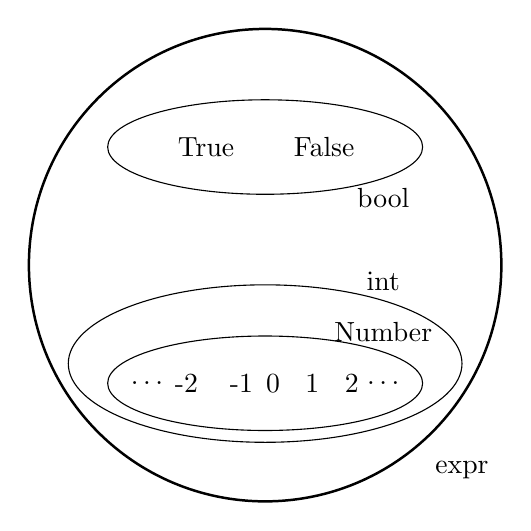
\begin{tikzpicture}




\draw[line width=0.9pt] (0,0) ellipse (3 and 3);
\node(expr) at (2.5, -2.6) {expr};

\draw (0,1.5) ellipse (2 and 0.6);
\node(bool) at (1.5, 0.85) {bool};
\node(true) at (-0.75, 1.5) {\code{True}};
\node(false) at (0.75, 1.5) {\code{False}};





\draw (0,-1.5) ellipse (2 and 0.6);
\node(Number) at (1.5, -0.85) {Number};
\node(int) at (1.5, -0.2) {int};
\draw (0,-1.25) ellipse (2.5 and 1);

\node(m3) at (-1.5, -1.5) {$\ldots$};
\node(m2) at (-1, -1.5) {\code{-2}};
\node(m1) at (-0.3, -1.5) {\code{-1}};
\node(0) at (0.1, -1.5) {\code{0}};
\node(1) at (0.6, -1.5) {\code{1}};
\node(2) at (1.1, -1.5) {\code{2}};
\node(3) at (1.5, -1.5) {$\ldots$};



\end{tikzpicture}

